\section*{Glosario}

\begin{itemize}
\item{\textbf{\'Etendue}}\\
\label{a1:etendue}
Es un par\'ametro que caracteriza c\'omo var\'ia la amplitud de la difusi\'on de un haz de luz, de acuerdo con el \'angulo abarcado o en la superficie iluminada. Es el producto de su area transversal (normal a la direcci\'on de propagaci\'on) y del \'angulo s\'olido que la subtiende.


\item{\textbf{PSF}}\\
\label{a1:psf}
Corresponde a la respuesta instrumental a una fuente de luz puntual, cuya radiaci\'on debe atravesar la atm\'osfera terrestre y los lentes del telescopio. La distorsi\'on puede ser interpretada como la convoluci\'on de la imagen por un kernel. \cite{huentelemu}. Ver imagen \ref{fig:a1}

\begin{figure}[h]
\centering
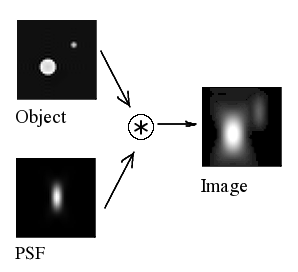
\includegraphics[scale=.5]{images/psf}
\caption{Ejemplo de distorsi\'on de una fuente al aplicar un kernel de PSF espec\'ifico. El resultado se observa en el cuado \textit{Image}.}
\label{fig:a1}
\end{figure}

\item{\textbf{Airmass}}\label{ap:airmass}\\
Es el largo del camino de que le toma a los rayos de una cuerpo celeste atravesar la atm\'osfera. A medida que los rayos van penetrando la atm\'osfera estos se van atenuando por la absorci\'on y el proceso conocido como scattering. 
\end{itemize}
\bigskip